
\(
\textbf{Probabilistic Path (PP):} 
\)
% The PP metric is another interesting property derived from our Markov transition matrix. Taking the product of the fundamental matrix F and the matrix of absorbing probabilities \(R\) results in a matrix, \(B = FR\), whose \(B(i,j) \) entries yield the probability of being absorbed by state \(s_j\) given we started at initial state \(s_i\).  


\begin{figure}[ht]
\centering
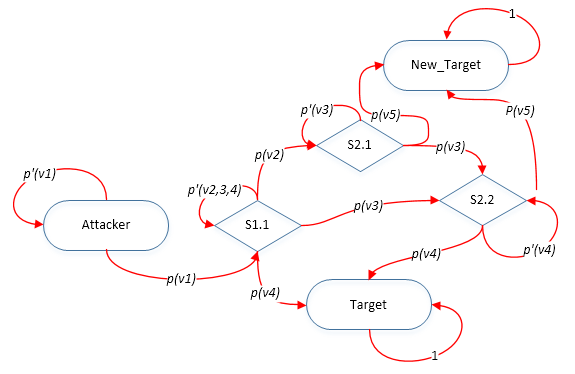
\includegraphics[width=.48\textwidth]{img/ag_extra_target.png}
\caption{Transition diagram with additional absorbing states New\_Target}
\label{fig:ag_pp}
\end{figure}


Recall that entries in the PP matrix \(B = FR\) produce the probability of being absorbed by state \(s_j\) from an initial state \(s_i\).  In the current scenarios we define a single attack target, so calculating this PP metric results in a column of 1’s due to absorbing markov chains requiring 100\% chance of absorption from any transient node by definition.   

However it is easy to imagine a case where multiple targets are specified in the model. For example, we have added a second absorbing state, ‘New\_Target’ to the transition diagram from Figure \ref{fig:ag_pp}. This could represent a hot failover clone of the existing Target or it could be a completely separate system with unique vulnerabilities. In either case we can make a grounded prediction on which state will absorb the attacker with the highest likelihood and prepare accordingly. 

